\section{Roughness propagation}
As described in section \ref{subsec:roughness_prop}, three different test cases
were setup to verify the propagation of the surface roughness values to the
correct volume cells.

\subsubsection{Cube}
This test was designed to make sure the propagation is sound. Figure
\ref{fig:cube_ks_prop} shows the surface cube with the rough patch in the middle
of each face. The volume mesh is sliced in two axis and the propagation of the
roughness values can be seen.

\begin{figure}[H] \centering
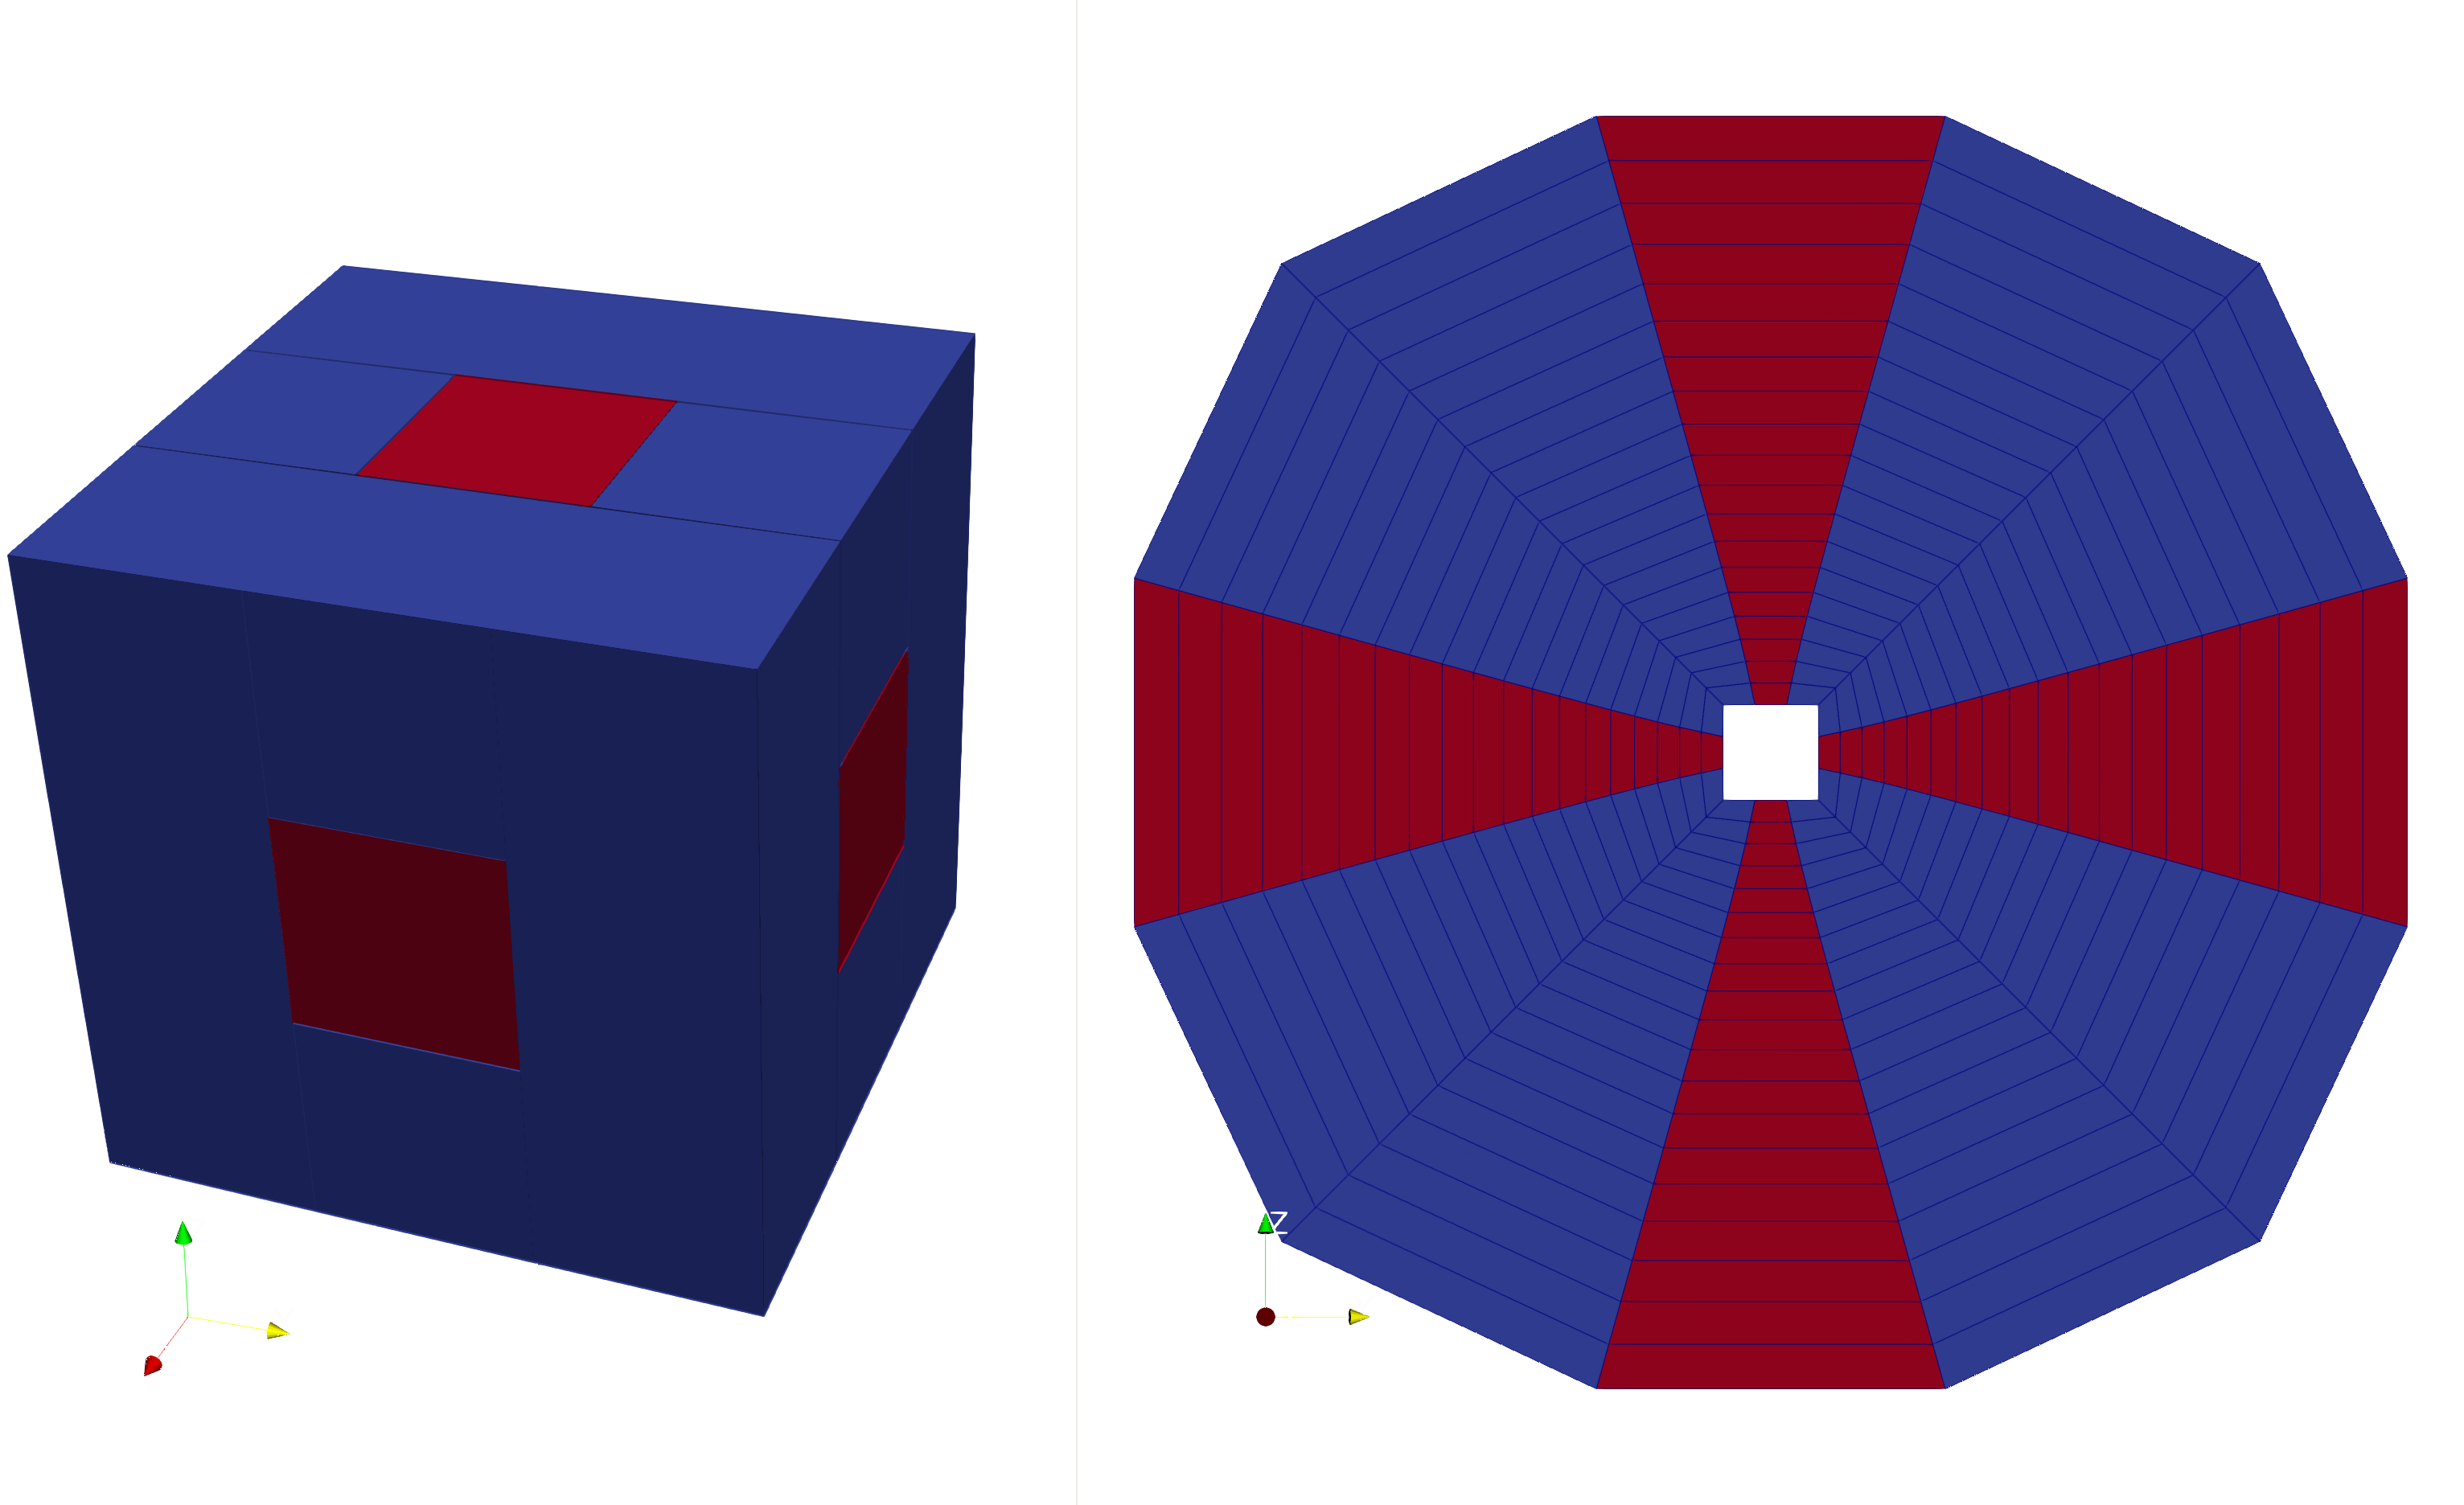
\includegraphics[width=0.5\textwidth]{cube_ks_prop.png}
    \caption{Cube with propagated roughness values. Red equals
$k_{s} = 1.0$ and blue $k_{s} = 0.1$.}
    \label{fig:cube_ks_prop}
\end{figure}

\subsubsection{Overset cube}
Similar to the previous test, is used to show that the roughness values are
propagated correctly for  overset meshes. As described in section
\ref{subsec:roughness_prop}, it was necessary to refine the mesh a bit. This was
needed as the \textit{implicit hole cutting} would fail otherwise. In figure
\ref{fig:cube_overset_ks_prop}, the two overlapping meshes with the correctly
propagated roughness values is shown.

\begin{figure}[H] \centering
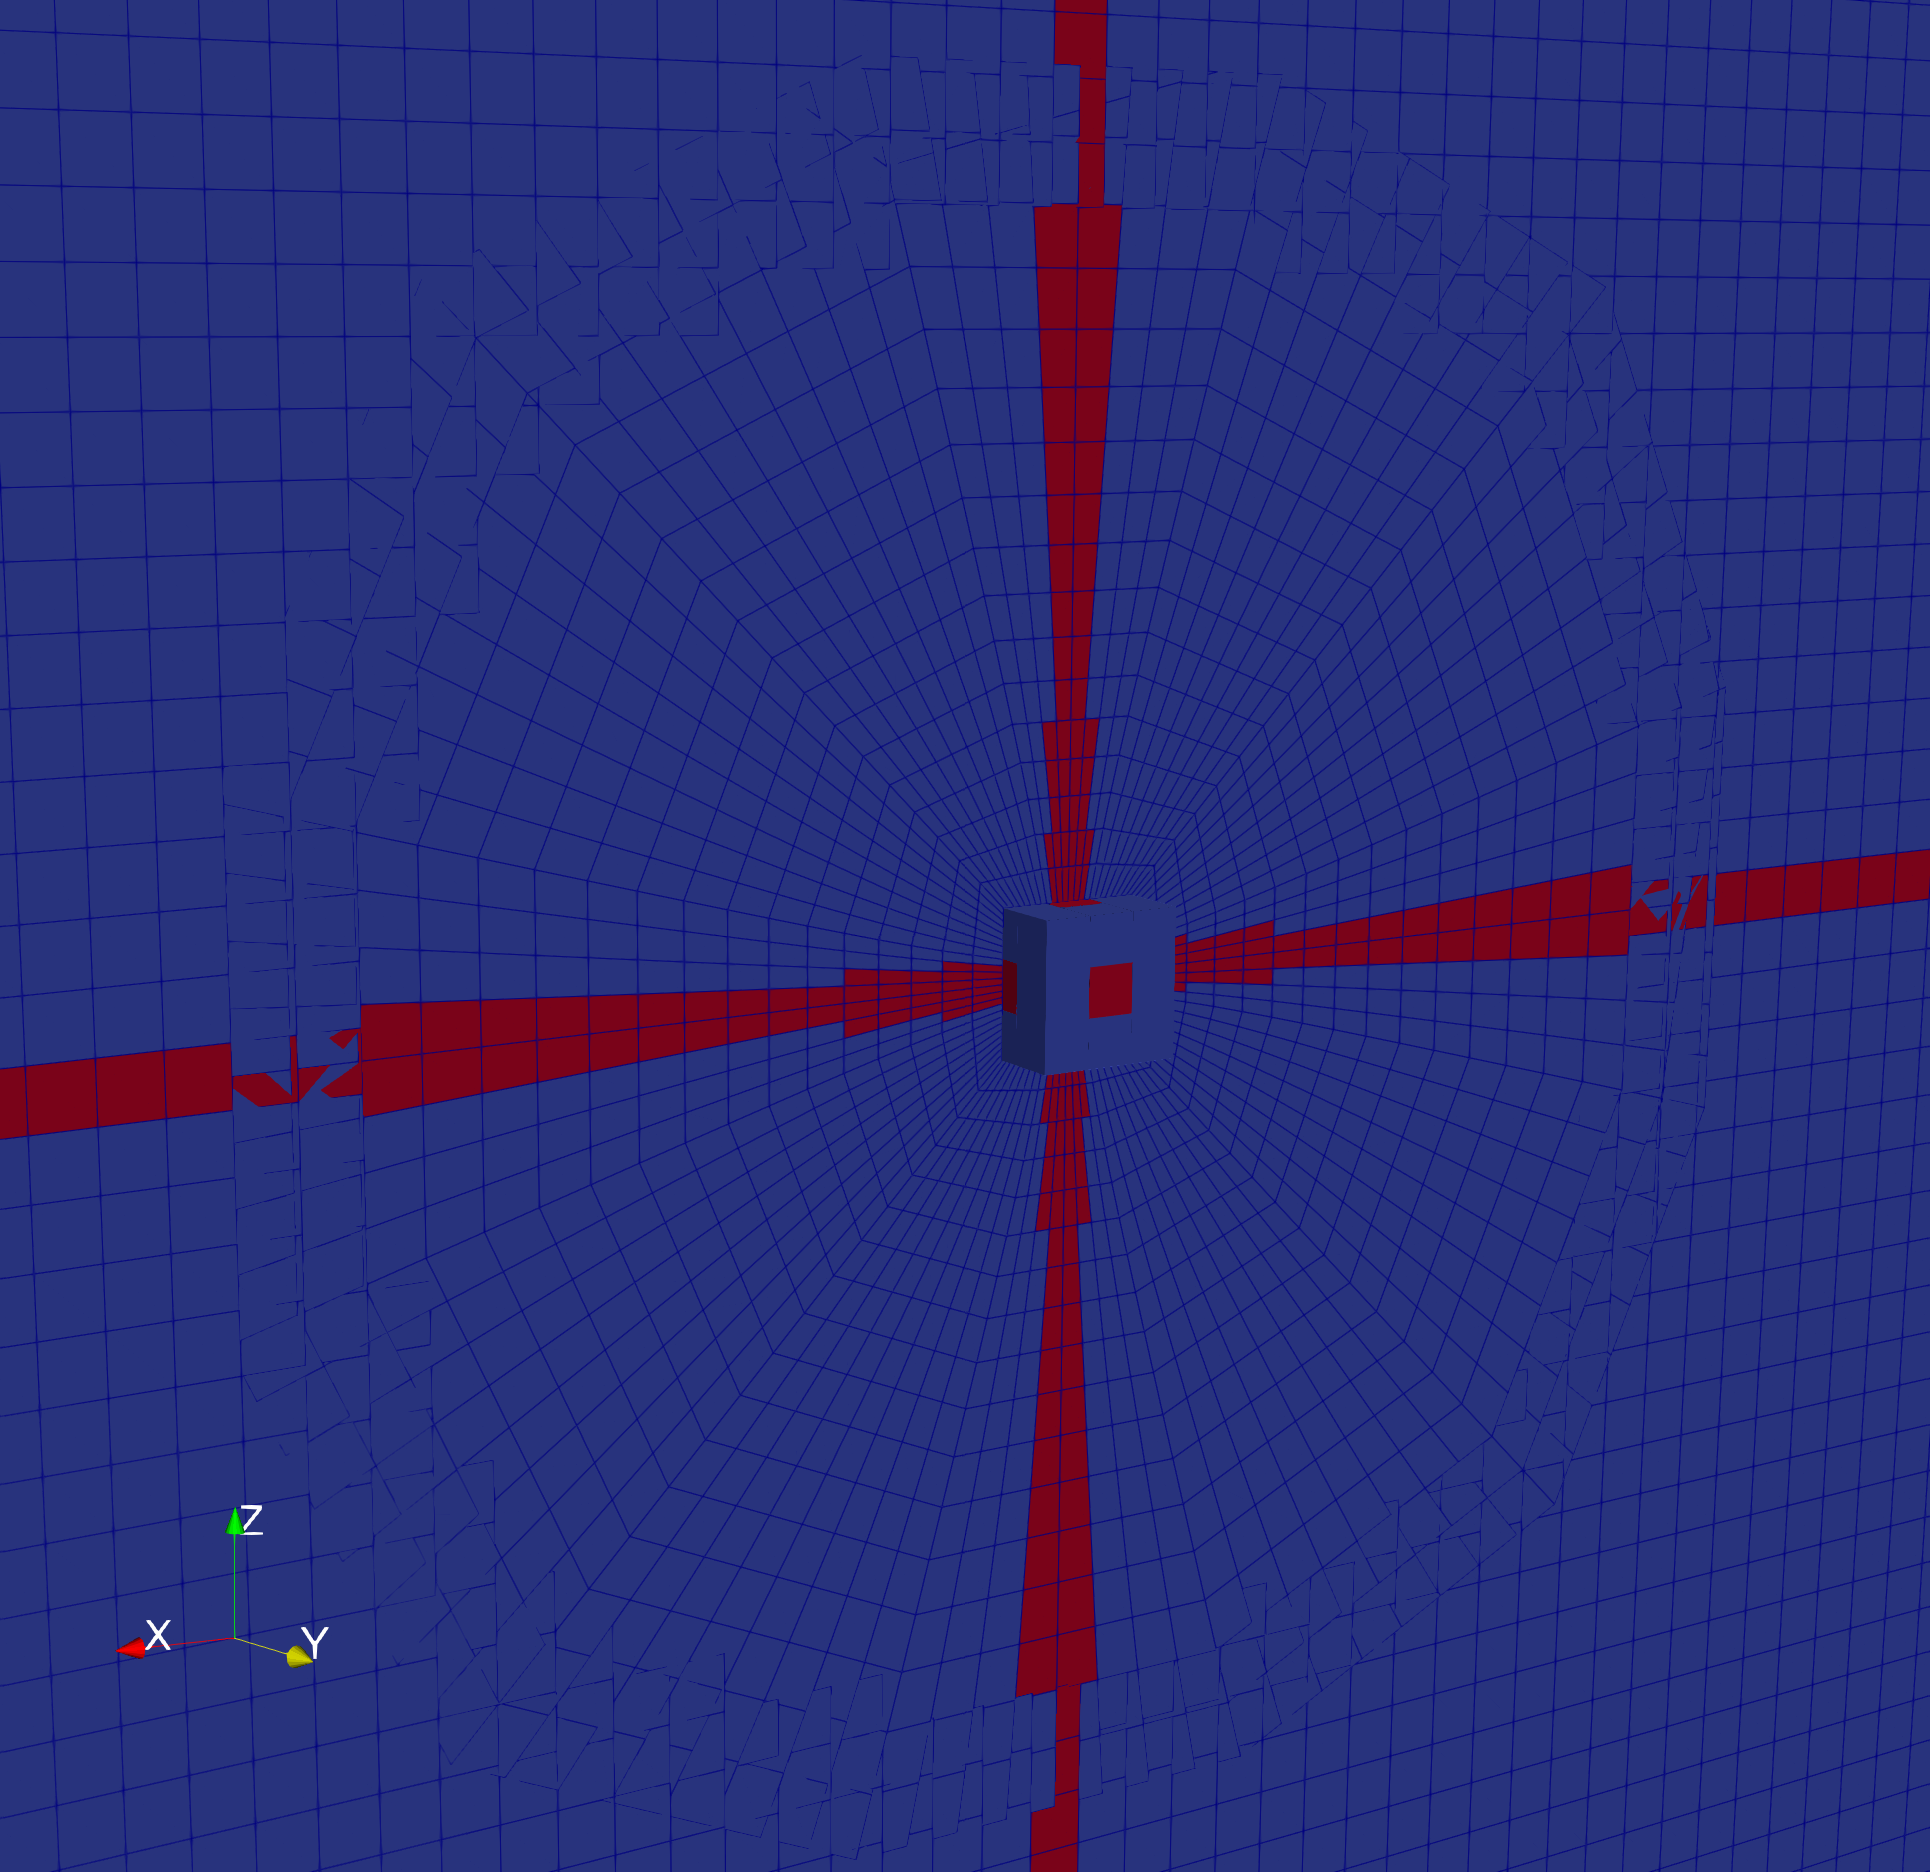
\includegraphics[width=0.5\textwidth]{cube_overset_ks_prop.png}
    \caption{Overset cube with propagated roughness values. Red equals
$k_{s} = 1.0$ and blue $k_{s} = 0.1$.}
    \label{fig:cube_overset_ks_prop}
\end{figure}

\subsubsection{Cuboid}
As described in section \ref{subsec:roughness_prop}, this 6 test cases were
designed to catch errors in the correlation of the surface cell to the global
cell index (\texttt{gID}). As such, no figures have been generated. But the
author is happy report that all tests have passed.

\section{Flap plate at zero incidence}

\subsubsection{Grid Convergence}
In figure \ref{fig:gc_rumsey_comp}, the grid convergence for various roughness
values is shown.  Additionally, grid convergence data for two different solvers
from \cite{rumsey_flat} is available for the skin friction coefficient. For
ADflow, the expected convergence rate is 2. When computing the actual ratio using equation
\ref{eq:conv_rate}, one gets a ratio of approximately 1. This is less than
expected and will be investigated further.

\begin{figure}[H] \centering
  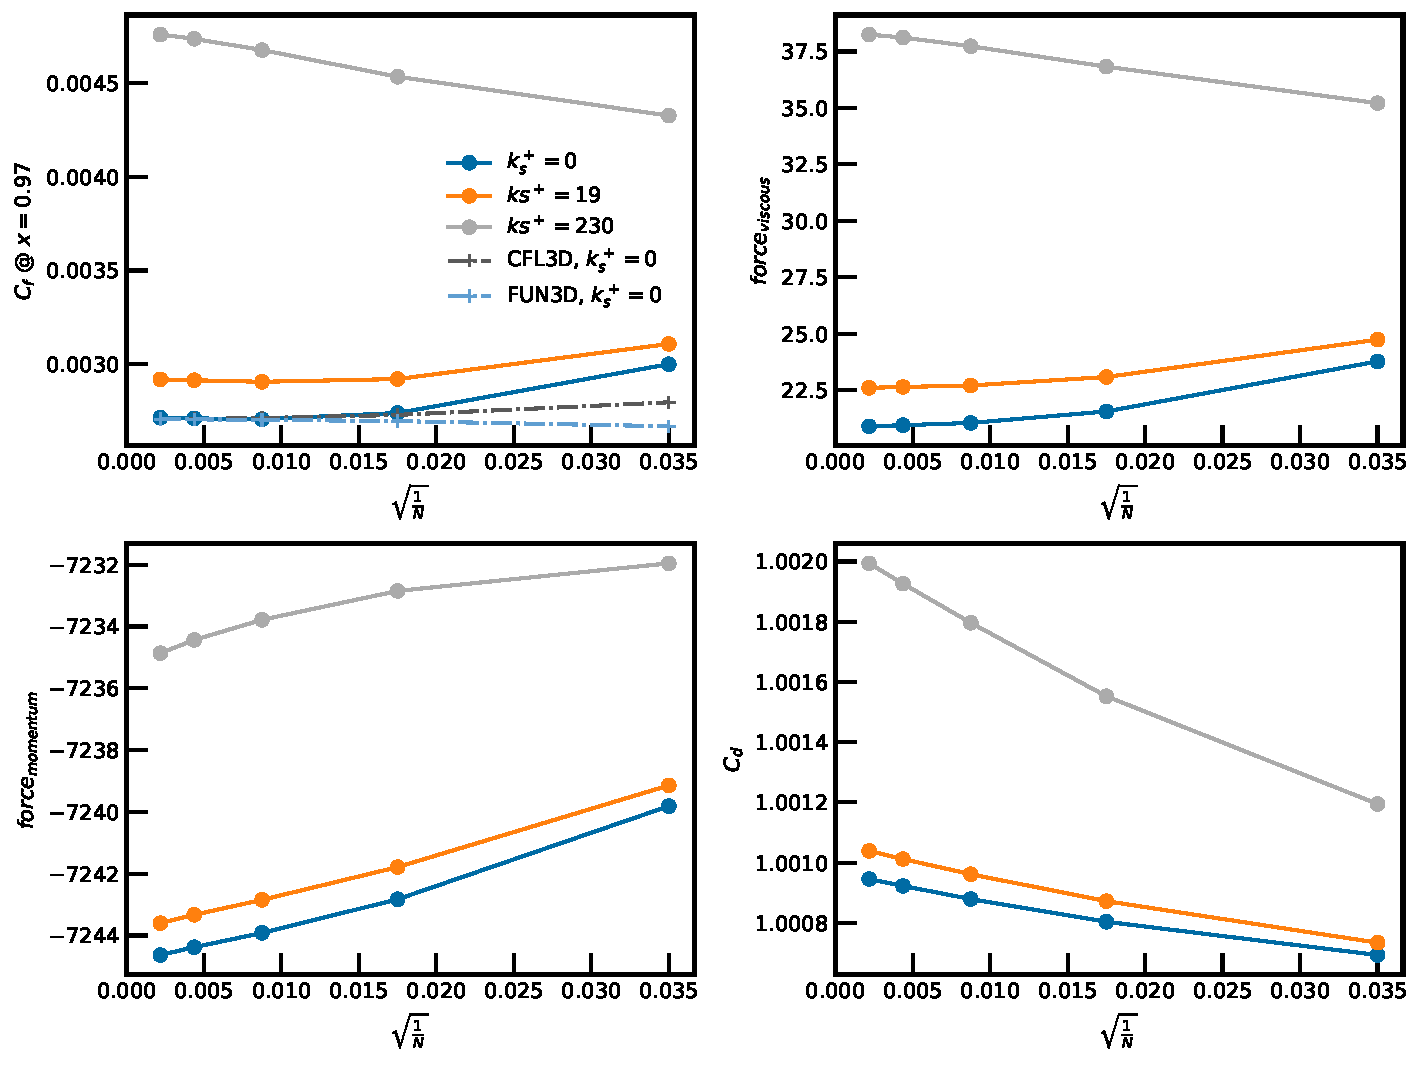
\includegraphics[width=0.9\textwidth]{comp/gc_rumsey_comp}
    \caption{Grid convergence for various roughness values. The skin friction
coefficient is overlayed with data from \cite{rumsey_flat}.}
    \label{fig:gc_rumsey_comp}
\end{figure}


\subsubsection{Clean}
In figure \ref{fig:cf_clean}, the skin friction coefficient over the flat plate
for a roughness value of $k_{s} = 0$ (clean) is shown. It is compared against
theory and data from the NASA tmr website \cite{rumsey_flat}. When looking
closely, ADflow and CFL3D agree well, but the theory is slightly off. The
agreement of both solvers indicates that the SA implementation is done correctly
(for a clean surface) in ADflow. The offset to theory probably means that the SA
model is not completely accurate in predicting the skin friction coefficient of
a flat plate.  It is unclear what the dip of the skin friction at the beginning
of the plate is. It may be explained as some kind of ``numerical'' transition. It
can be observed in other plots as well, but only for ADflow.

\begin{figure}[H] \centering
  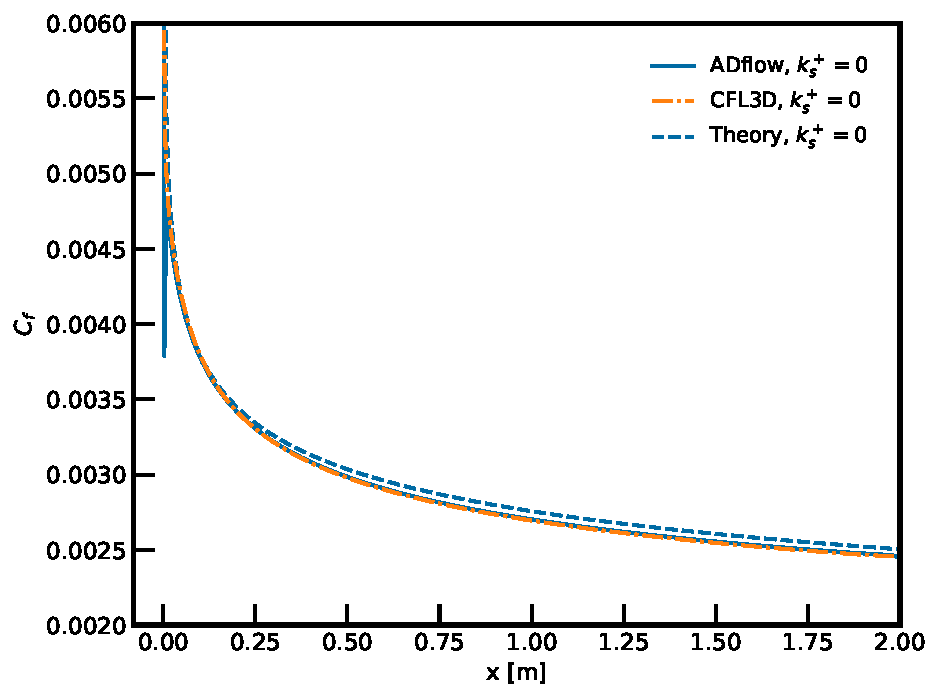
\includegraphics[width=0.6\textwidth]{comp/cf_clean}
    \caption{Skin friction coefficient for a roughness value of $k_{s} = 0$
      compared against theory and data from \cite{rumsey_flat}.}
    \label{fig:cf_clean}
\end{figure}

\noindent In figure \ref{fig:vp_clean}, the velocity profile at different
positions on the flat plate is plotted. It is compared against theory and
reference data from CFL3D. All curves agree extremely well.
\begin{figure}[H] \centering
  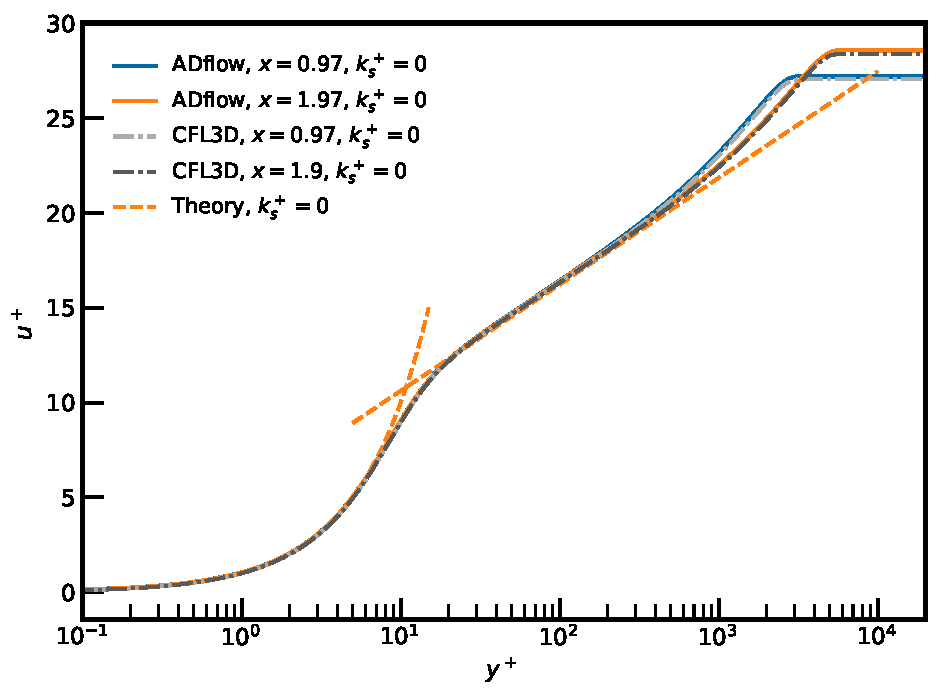
\includegraphics[width=0.6\textwidth]{comp/vp_clean}
    \caption{Velocity profile for a roughness value of $k_{s} = 0$ compared
      against theory and  data from \cite{rumsey_flat}.}
    \label{fig:vp_clean}
\end{figure}

\subsubsection{Blanchard}
In figure \ref{fig:cf_blanchard}, the skin friction coefficient for the clean
case and a roughness value of $k_{s}^{+} = 150$ is plotted. The clean case is
compared against theory and the rough against experimental data from Blanchard's
PhD thesis. But (as described in section \ref{subsec:flat_plate_exp}), the data
has been extracted from a different source \cite{sa_rough}. The theory and clean
case agree well, but the rough case does not. The ``numerical'' transition is
more obvious for the clean case. It also exists for the rough case, but is
seemingly inverted.

\begin{figure}[H] \centering
  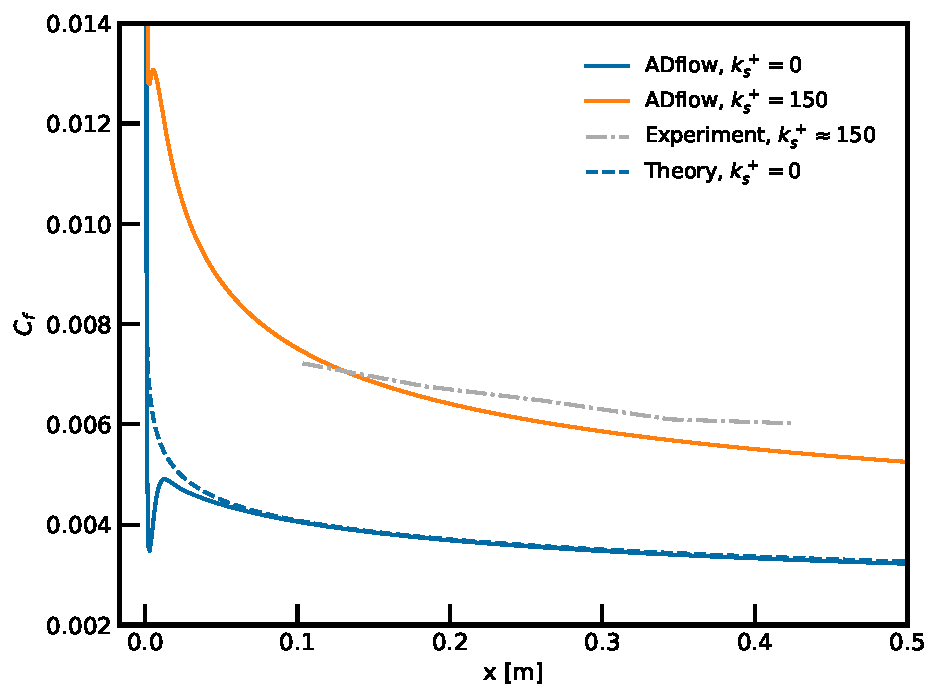
\includegraphics[width=0.6\textwidth]{comp/cf_blanchard}
    \caption{Skin friction coefficient for various roughness values compared
      against theory and SU2.}
    \label{fig:cf_blanchard}
\end{figure}


\subsubsection{Acharya et al.}
In figure \ref{fig:cf_acharya}, the skin friction coefficient for various
roughness values are plotted against theory and two experiments from
\cite{Acharya1986}. As before, the theory and clean case agree well. But the
rough cases do not. First of all, the skin friction coefficient is
under-predicted for ADflow. Coincidentally, the simulation for case two aligns
with case one. When ignoring the offset, one can conclude that at least the
predicted shape matches. The two curves do not agree at the beginning, but this
may be explained through transitional effects as the SA model is fully
turbulent. The ``numerical'' transition is again observable at the beginning of
the plate.

\begin{figure}[H] \centering
  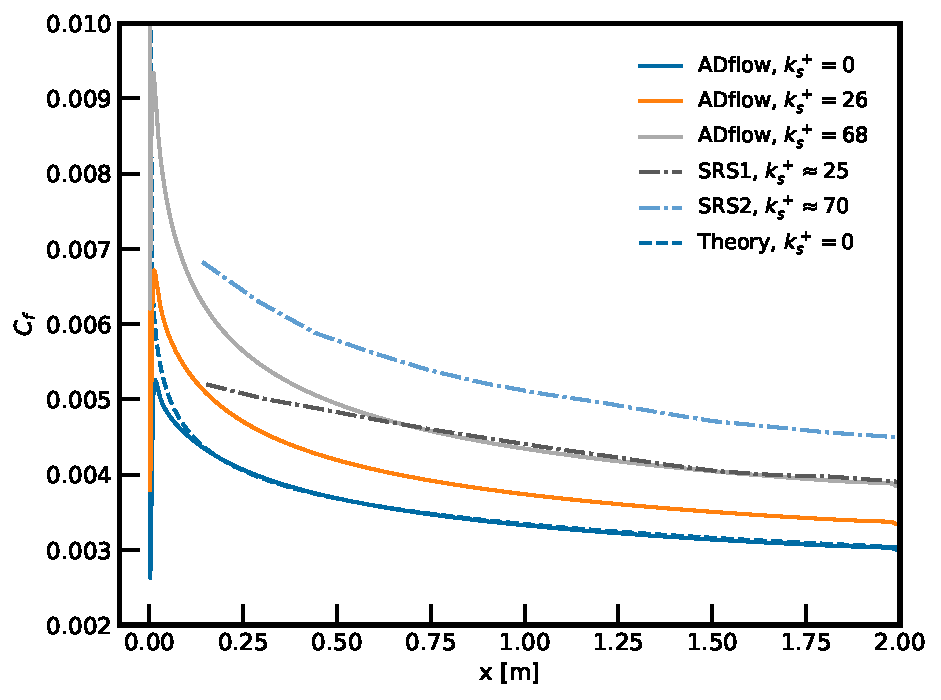
\includegraphics[width=0.6\textwidth]{comp/cf_acharya}
    \caption{Skin friction coefficient for various roughness values compared
      against theory and experimental data from \cite{Acharya1986}.}
    \label{fig:cf_acharya}
\end{figure}

\noindent In figure \ref{fig:vp_acharya}, the velocity profile for various
roughness values is plotted against theory and experimental data. Theory does
agree well for the clean case, but there is a big offset for the rough case.
ADflow values are not shifted enough. This indicates an underprediction of the
roughness effects which is consistent with the underprediction of the skin
friction coefficient. When looking at the experimental data, one can also
observe a slight underprediction. But this is explainable through the use of
mean values measured. This means, this curve also includes contributions from
places where the boundary layer has not fully developed.

\begin{figure}[H] \centering
  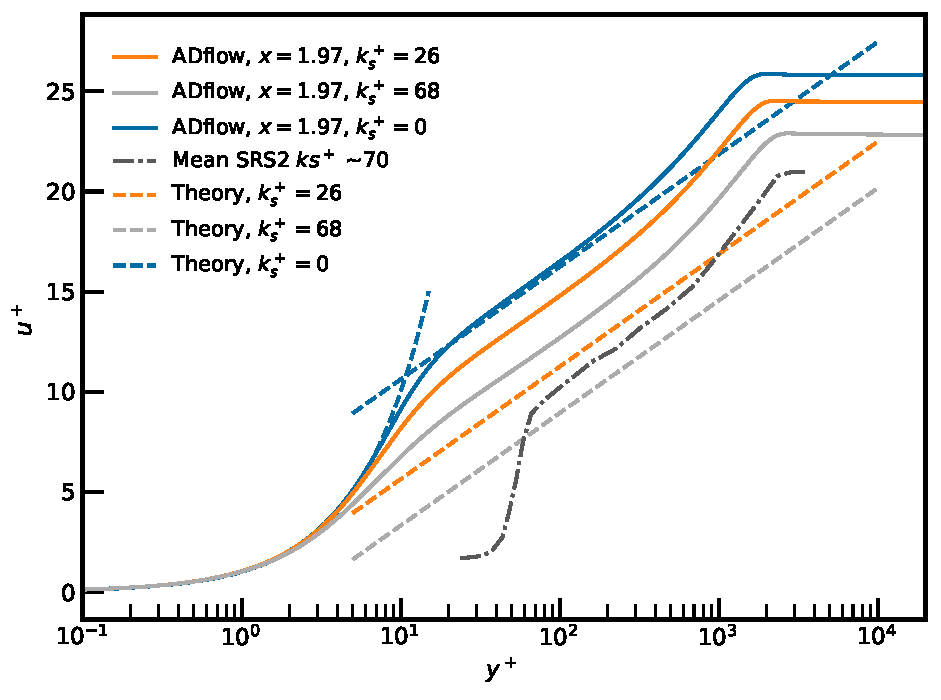
\includegraphics[width=0.6\textwidth]{comp/vp_acharya}
    \caption{Velocity profile for various roughness values compared
      against theory and experimental data from \cite{Acharya1986}.}
    \label{fig:vp_acharya}
\end{figure}



\subsubsection{SU2}
To validate the implementation itself, the skin friction coefficient for various
roughness values is plotted against data from SU2. For the clean case, both
solvers agree well. But for the rough cases, one can observe the same offset as
seen before. For ADflow, the ``numerical'' transition can be seen clearly at the
beginning. For SU2, it is obscured, but the author is happy to report that it
does not exist.

\begin{figure}[H] \centering
  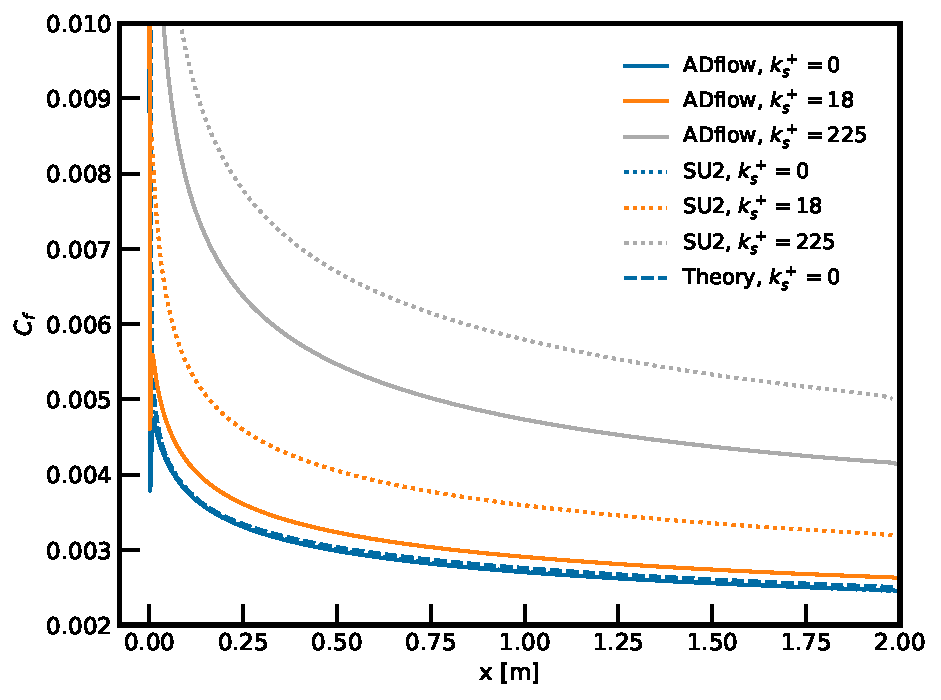
\includegraphics[width=0.6\textwidth]{comp/cf_rumsey_comp}
    \caption{Skin friction coefficient for various roughness values compared
      against theory and SU2.}
    \label{fig:cf_rumsey_comp}
\end{figure}

\noindent In figure, \ref{fig:vp_rumsey_comp}, the velocity profile for
different roughness values is shown. For the clean case, both solvers agree well
with theory. SU2 does also agree well for the rough cases although having a
slight offset. For ADflow, the same shift compared to SU2 and theory is
observable.

\begin{figure}[H] \centering
  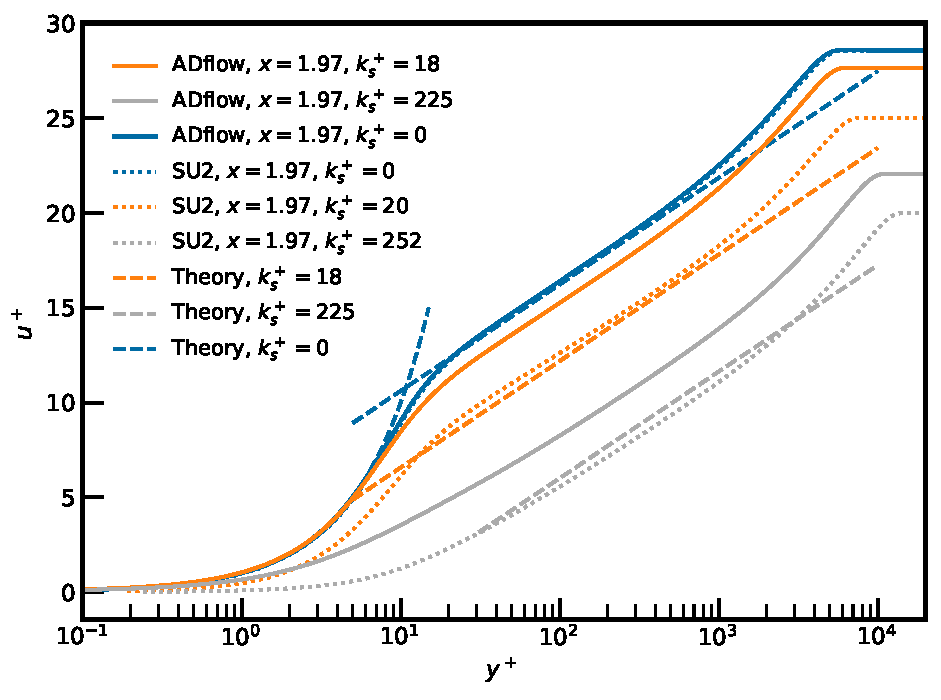
\includegraphics[width=0.6\textwidth]{comp/vp_rumsey_comp}
    \caption{Velocity profile for various roughness values compared
      against theory and SU2.}
    \label{fig:vp_rumsey_comp}
\end{figure}

\subsection{Offset}
As has been shown in the last section, the SA rough implementation in ADflow is
somehow not correct. It is observable that the predicted shape of the curves is
correct, but they seem to be offset compared to experiments and SU2. At the time
of writing it is not clear what is causing this, but it will be investigated
further.

\section{Automated tests} Reporting the results of the automated tests is
easiest done in tabular form.
Thus, take a look at table \ref{tab:tests_results}.


\begingroup
\renewcommand{\arraystretch}{1.5} % adjust vertical spacing
\begin{xltabular}{\textwidth}{lX}
    \toprule
    Test-Name                                     & Comment \\
    \toprule
    \endhead
    \texttt{TestAdjoint\_5\_Rough\_SA\_wing}      & \\

    $\rightarrow$ \texttt{rest\_residuals}        & Passes to an absolute and
    relative tolerance of \num{1e-10}. \\

    $\rightarrow$ \texttt{rest\_adjoint}           & Passes to an absolute and
    relative tolerance of \num{1e-10}. \\

    \midrule

    \texttt{TestCmplxStep\_5\_Rough\_SA\_wing}    & \\

    $\rightarrow$ \texttt{cmplx\_test\_aero\_dvs} & Passes to an absolute
tolerance of \num{5e-10} and a relative tolerance of \num{1e-8}. \\

    $\rightarrow$ \texttt{cmplx\_test\_geom\_dvs}& Fails with an absolute and relative
    tolerance of \num{5e-9} as follows\footnote{All functionals are only listed
      for \textit{span} as it does not provide much more additional insight.}:

    \begingroup
    \renewcommand{\arraystretch}{1.0} % adjust vertical spacing
    \begin{tabular}{l l r r}
      Functional & design var. & abs. tol.      & rel. tol. \\
      \toprule
      $C_{l}$    & span        & \num{1.64e-8}  & \num{3.77e-7} \\
      $C_{d}$    & span        & \num{9.39e-9}  & \num{6.44e-6} \\
      $C_{mz}$   & span        & \num{2.62e-8}  & \num{4.10e-7} \\
      lift       & span        & \num{6.67e-3}  & \num{3.77e-7} \\
      drag       & span        & \num{4.42e-4}  & \num{4.73e-7} \\
      $C_{l}$    & twist       & \num{7.21e-9}  & \num{2.92e-7} \\
      $C_{l}$    & shape       & \num{2.29e-7}  & \num{3.45e-4} \\

    \end{tabular}
    \endgroup

    \\

    \midrule

    \texttt{TestFunctionals\_9\_Rough\_SA\_wing} & \\

    $\rightarrow$ \texttt{rest\_residuals}        & Passes to an absolute and
    relative tolerance of \num{1e-10}. \\

    $\rightarrow$ \texttt{rest\_restart\_read}    & Passes to an absolute and
    relative tolerance of \num{1e-10}. \\

    $\rightarrow$ \texttt{rest\_functions}        & Passes to an absolute and
    relative tolerance of \num{1e-9}. \\

    $\rightarrow$ \texttt{test\_forces\_and\_tractions} & Passes to an absolute and
    relative tolerance of \num{1e-10}. \\

    $\rightarrow$ \texttt{test\_jac\_vec\_prod\_fwd} & Passes to an absolute and
    relative tolerance of \num{5e-9}. \\

    $\rightarrow$ \texttt{test\_jac\_vec\_prod\_bwd} & Passes to an absolute and
    relative tolerance of \num{1e-10}. \\

    $\rightarrow$ \texttt{test\_dot\_products} & Passes to an absolute and
    relative tolerance of \num{1e-10}. \\

    \midrule

    \texttt{TestFunctionals\_10\_Rough\_SA\_rans\_tut\_wing} & All tests pass.
    The tolerances are the same as for
    \texttt{TestFunctionals\_9\_Rough\_SA\_wing} listed above.\\

  \bottomrule

  \caption{Results for automated tests.}
  \label{tab:tests_results}
\end{xltabular}
\endgroup


\noindent All tests passing except for the geometric design variables in
\texttt{TestCmplxStep\_5\_Rough\_SA\_wing} indicates that there is something
wrong with the Automatic Differentiation. Although it is important to point out
the size of the relative error at \num{1e-7} is already quite small. The
\textit{finite differences} approach could only yield such an accurate gradients
when finding the perfect step length, which is not to be expected. This will
also be investigated further.
